%
%	Begrifflichkeiten
%

\pagebreak
\section{Business Model Innovation}

\onehalfspacing

\subsection{Business Model}

First, we need to define what a business model might be.

In dialectical materialism, the philosophical movement developed by Karl Marx and Friedrich Engels, the world is explained in a materialistic manner, i.e., starting from material conditions.\footnote{See \textit{MIA (2022)}: Encyclopedia of Marxism. \cite{diaMat}}

Dialectical materialism uses the dialectical method, hence the name, which views contradictions and change as the driving force behind development. There are no direct "business models" in the sense of today's economic concepts that can be derived from dialectical materialism. However, certain principles of dialectical materialism can be applied to the analysis of business models to understand their contradictions and potential for development.

The dialectical method helps to analyze the development of a business model and to understand how quantitative changes (e.g., growth) can lead to qualitative leaps (e.g., new business areas). A business model can also be negated by external influences (e.g., technological innovations) or internal developments (e.g., strategic realignment) and replaced by a new one.

In our case, dialectical materialism will help us understand the influence of adversarial external factors, such as COVID-19, on the business model of FOM and the decision to develop DLS.

\subsection{Business Model Canvas}

A more traditional tool to analyze and understand a business model is the Business Model Canvas, created by Alexander Osterwalder.\footnote{See \textit{Osterwalder, A. (2011)}: Business Model Generation. \cite{alexBmc}}

It's a strategic management tool that provides a visual framework for developing, describing, and analyzing business models; it's displayed on a single page divided into nine key building blocks:

\begin{itemize}
    \item Key Partners
    \item Key Activities
    \item Key Resources
    \item Value Propositions
    \item Customer Relationships
    \item Channels
    \item Customer Segments
    \item Cost Structures
    \item Revenue Streams
\end{itemize}

With the change in perception of remote work, the perception of distance learning also changed, and thus allowed for a revised value proposition for learning at FOM.

\subsection{Business Model System}

Another model, the Business Model System,  refers to the interconnected network of relationships, processes, and stakeholders that work together to create, deliver, and capture value within and around a business model. It's a more dynamic and comprehensive view than static frameworks like the Business Model Canvas.\footnote{\textit{Tewes, S. (2020)}: Geschäftsmodelle neu denken. \cite{zukunft}} 

\begin{figure}[H]
\centering
\caption {Business Model System}
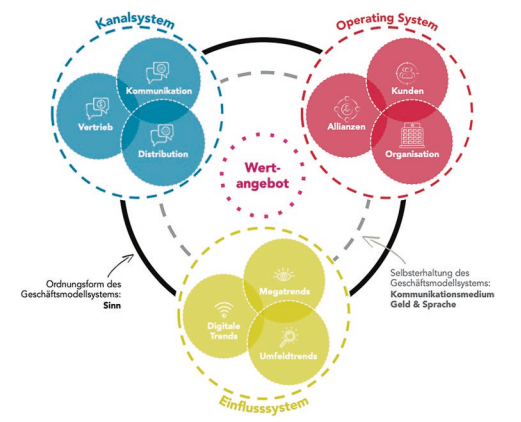
\includegraphics[width=\linewidth]{images/business-model-system.png}
\label{fig:businessModelSystem}
\end{figure}

Here, we also have at the center of the system the value proposition that FOM had to change after COVID-19.
